%{\color{red}
%\begin{itemize}
%\item New memory technologies
%\item Why is virtual address shared space is a challenge with the advent of
%these new technologies
%
%\item How is CPU--GPU space changing in terms
%of high bandwidth but lower latency interconnects
%\item Present opportunities and challenges
%\item Combine intro of first 3 GPU papers
%
%\item Google Proposal
%\item How cheaper but slower mem technologies can lead to boosting perf/dollar
%in data-centers
%\item Present opportunities and challenges
%\end{itemize}
%}
%
The emergence of {\it heterogeneous memory systems} has resulted in a need for
new memory management policies that are able to fully exploit these systems.
While traditional memory management techniques largely assume a ``homogeneous''
main memory, future systems are likely to have two or more different types of
main memories attached to them -- thus the term ``heterogeneous'' memory
systems. Examples of such systems are the recently announced GPUs
 \cite{pascal}, which are slated to have high bandwidth connection to the host
CPU by NVLink~\cite{NVLINK} and thus can access host memory seamlessly.  Another
example is Intel's 3-D XPoint~\cite{xpoint} technology that provides a slow but
cheaper and large capacity non-volatile memory (NVRAM) along with a regular DRAM
based memory attached to the same CPU node.  There are several aspects of such
memory technologies that have not been studied before:

a) \textbf{Different bandwidths:}
Different memory technologies will typically have huge differences in their
bandwidths, e.g., a GPU connected to on-board GDDR and host-side DDR memories
can have a bandwidth differential of $\approx$ 2 -- 8 $\times$ between the two
memory technologies. Since GPUs are very sensitive to main memory bandwidth, the
metric to optimize for in such systems is the total available bandwidth to the
GPU from the two memory sources. While prior work on Non-Uniform Memory Access
(NUMA) has closely looked at data placement strategies to optimize the total
memory {\it access latency} in the presence of different memory banks with
different access latencies, we show that such policies are not suited to
optimizing the total memory {\it bandwidth}. Instead, we propose {\it
Bandwidth-Aware Placement} (BW-AWARE), which directly maximizes the overall
bandwidth, and show that it can significantly increase application throughput
for several GPU applications.

b) \textbf{Different coherency domains:} 
In a heterogeneous CPU-GPU memory system, implementing hardware cache coherence
between the CPU and the GPU can lead to a significant challenges because of
design and verification involved particularly if the two domains are designed by
separate vendors. We introduce {\it Selective Caching}, a coherence policy that
disallows GPU caching of any memory that would require coherence updates to
propagate across the two domains. This approach decouples the cache-coherence
protocols in CPUs and GPUs, thus improving cross-vendor design cycle time.

c) \textbf{Different costs per bit:}
Different memory technologies can have different costs.  For example, recently
announced non-volatile memory technology~\cite{xpoint} is projected to be
significantly cheaper than regular DRAM, while also being significantly higher
latency. Their lower cost per bit makes them a good candidate for use in
data-centers, where main memory cost can be up to $\approx$ 30\% of the total
cost of ownership (TCO). However, their low speed means that only {\it cold},
i.e., infrequently accessed data can be placed in such memories.  Placing more
cold data in the slower memories conflicts with efficient virtual memory usage
by transparent huge page (THP), which can provide 10-15\% performance gains in
large memory footprint data-center applications. We study how to reap the
benefits of huge pages while also placing as much data in slow memory as
possible, to improve performance per dollar at data-center scale.

Below, we describe each of these three problems in detail and give a brief
sketch of our proposed solution to these problems.

\section{Bandwidth-asymmetric Systems}
To date, GPU-attached Bandwidth-Optimized (BO) memory has been allocated and
managed primarily as the result of explicit, programmer-directed function calls.
To make best use of the bandwidth available to GPU programs, programmers
manually copy the data over the relatively slow PCIe bus to the GPU memory, and
-- only then -- launch their GPU kernels.  This up-front data allocation and
transfer has been necessary since transferring data over the PCIe bus is a high
overhead operation, and a bulk transfer of data amortizes this overhead. This
data manipulation overhead also results in significant porting challenges when
retargeting existing applications to GPUs, particularly for high-level languages
that make use of libraries and dynamic memory allocation during application
execution.

\begin{figure}[t]
    \centering
    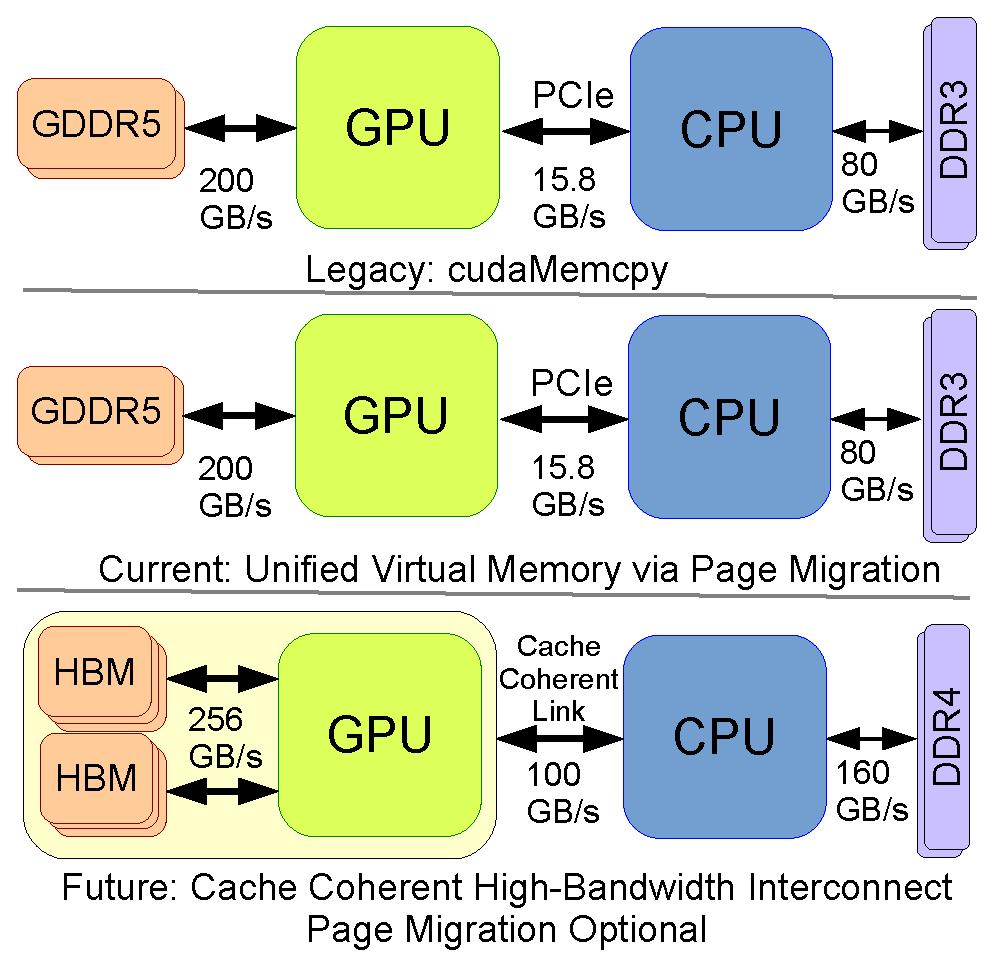
\includegraphics[width=0.7\columnwidth]{hpca2015/figures/architecture.eps}
    \caption{System architectures for legacy, current, and future mixed GPU-CPU systems.}
    \label{fig:arch-hpca2015}
\end{figure}

Recognizing the obstacle this programming model poses to the wider adoption of
GPUs in more parallel applications, programming systems like NVIDIA's CUDA,
OpenCL, and OpenACC are evolving to shared virtual address space between CPU and
GPU. Concurrently, CPU-GPU architectures are evolving to have unified globally
addressable memory systems in which both the GPU and CPU can access any portion
of memory at any time, regardless of its physical location.  Today this unified
view of memory is layered on top of legacy hardware designs by implementing
software-based runtimes that dynamically copy data on demand between the GPU and
CPU~\cite{cuda}. As depicted in Figure~\ref{fig:arch-hpca2015}, over the next
several years it is expected that GPU and CPU systems will move away from the
PCIe interface to a fully cache coherent (CC) interface ~\cite{AMDHSA}. These
systems will provide high bandwidth and low latency between the non-uniform
memory access (NUMA) pools attached to discrete processors by layering coherence
protocols on top of physical link technologies such as NVLink~\cite{NVLINK},
Hypertransport~\cite{AMDHT}, or QPI~\cite{INTELQPI}.   CC-NUMA access to
CPU-attached memory from the GPU makes the software page migration used today an
optional feature thanks to the improved bandwidth, latency, and access
granularity that cache coherence can provides.

As heterogeneous CPU-GPU systems move to a transparent unified memory system,
the OS and runtime systems need information about other aspects of memory zones
such as their bandwidths instead of only the access latency information that is
exposed today via Advanced Configuration and Power Interface (ACPI). In CC-NUMA
systems today, latency information alone is adequate as CPUs are generally more
performance sensitive to memory system latency rather than other memory
characteristics. In contrast, massively parallel GPUs and their highly-threaded
programming models have been designed to gracefully handle long memory
latencies, instead demanding high bandwidth. Unfortunately, differences in
bandwidth capabilities, read versus write performance, and access energy are not
exposed to software; making it difficult for the operating system, runtime, or
programmer to make good decisions about memory placement in these GPU-equipped
systems. In this thesis we investigate the effect on GPU performance of exposing
memory system bandwidth information to the operating system/runtime and user
applications to improve the quality of dynamic page placement and migration
decisions.

\section{Different Coherence Domains}
%Technology trends indicate an increasing number of systems designed with CPUs,
%accelerators, and GPUs coupled via high-speed links. Such systems are likely to
%introduce unified shared CPU-GPU memory with shared page tables. In fact, some
%systems already feature such implementations~\cite{AMDKaveri}.
Introducing globally visible shared memory improves programmer productivity by
eliminating explicit copies and memory management overheads. Whereas this
abstraction can be supported using only software page-level protection
mechanisms~\cite{UVM, HSA}, hardware cache coherence can improve performance by
allowing concurrent, fine-grained access to memory by both CPU and GPU.
%If the CPU and GPU have separate physical memories, page migration may also be
%used to optimize page placement for latency or bandwidth by using both near and
%far memory~\cite{Dashti2013,Agarwal2015b,Meswani2015,Chou2015}.

%Some CPU--GPU systems will be tightly integrated into a system on chip (SoC)
%making on-chip hardware coherence a natural fit, possibly even by sharing a
%portion of the on-chip cache hierarchy~\cite{HSA,AMDAPU,Hechtman2014}.  However,
%the largest GPU implementations consume nearly 8B transistors and have their own
%specialized memory systems~\cite{NVIDIA8BILLION}.  Power and thermal constraints
%preclude single-die integration of such designs.  Thus, many CPU--GPU systems
%are likely to have discrete CPUs and GPUs connected via dedicated off-chip
%interconnects like NVLINK (NVIDIA), CAPI (IBM), HT (AMD), and QPI (INTEL) or
%implemented as multi-chip modules~\cite{NVLINK,CAPI,AMDHT,INTELQPI,Chen92}.
%The availability of these high speed off-chip interconnects has led both
%academic groups and vendors like NVIDIA to investigate how future GPUs may
%integrate into existing OS controlled unified shared memory regimes used by
%CPUs~\cite{Pichai2014,Power2014,Agarwal2015,Agarwal2015b}.

Current CPUs have up to 18 cores per socket~\cite{INTELXEONE5V3} but GPUs are
expected to have hundreds of streaming multiprocessors (SMs) each with its own
cache(s) within the next few years. Hence, extending traditional hardware
cache-coherency into a multi-chip CPU-GPU memory system requires coherence
messages to be exchanged not just within the GPU but over the CPU-GPU
interconnect. Keeping these hundreds of caches coherent with a traditional HW
coherence protocol, as shown in Figure~\ref{fig:motivation}, potentially
requires large state and interconnect bandwidth~\cite{Kelm2010,johnson2011}.
Some recent proposals call for data-race-free GPU programming models, which
allow relaxed or scoped memory consistency to reduce the frequency or hide the
latency of enforcing coherence~\cite{Hechtman2014}.  However, irrespective of
memory ordering requirements, such approaches still rely on hardware
cache-coherence mechanisms to  avoid the need for software to explicitly track
and flush modified cache lines to an appropriate scope at each synchronization
point. Techniques like region coherence~\cite{Power2013} seek to scale coherence
protocols for heterogeneous systems, but require pervasive changes throughout
the CPU and GPU memory systems. Such approaches also incur highly coordinated
design and verification effort by both CPU and GPU vendors~\cite{Hong2012} that
is challenging when multiple vendors wish to integrate existing CPU and GPU
designs in a timely manner.

Due to the significant challenges associated with building such cache-coherent
systems, in this thesis, we architect a GPU \textit{selective caching} mechanism.
This mechanism provides the conceptual simplicity of CPU-GPU hardware cache
coherence and maintains a high level of GPU performance, but does not actually
implement hardware cache coherence within the GPU, or between the CPU and GPU.
%In our proposed selective caching GPU, the GPU does not cache data that resides
%in CPU physical memory, nor does it cache data that resides in the GPU memory
%that is actively in-use by the CPU on-chip caches.
%This approach is orthogonal to the memory consistency model and leverages the
%latency tolerant nature of GPU architectures combined with upcoming low-latency
%and high-bandwidth interconnects to enable the benefits of shared memory.

\section{Proposal: Cheaper Memory Technologies}
Upcoming memory technologies, such as Intel's recently-announced XPoint-3D
memory~\cite{xpoint}, are projected to be denser and cheaper per bit than DRAM
while providing the byte-addressable load-store interface of conventional main
memory.  Improved capacity and cost per bit comes at the price of higher access
latency, projected to fall somewhere in the range of 500ns to several
microseconds.  The impending commercial availability of such devices has renewed
interest in two-tiered physical memory, wherein part of a system's physical
address space is implemented with the slower, cheaper memory technology.  Slow
memory can result in a net TCO win if the cost savings of replaced DRAM outweigh
cost increase due to reduced program performance or by enabling a higher peak
memory capacity per server than is economically viable with DRAM alone.  

%Our preliminary results indicate that over half of the memory footprint of
%representative cloud applications (e.g., Cassandra) are identified as cold by
%Linux’s kstaled mechanism, indicating that the corresponding pages have an
%inter-access interval exceeding 120s.  Analytic modeling suggests these pages
%could be shifted to a memory with a 3us access time with negligible (<3\%)
%performance degradation.

%%It's an interesting problem
%Prior academic work has considered two approaches to two-tiered memory: via a
%paging mechanism~\cite{1,2}, wherein accesses to slow memory invoke a page fault that
%must transfer data to fast memory before an access may proceed, and via a
%migration mechanism (as in cache coherent NUMA multiprocessors)~\cite{XXX}, wherein no
%software fault is required.  In the latter scenario, a migration mechanism seeks
%to shuffle pages between tiers to maximize fast-memory accesses.  

%It's an unsolved problem
Prior academic work on two-tiered memory has assumed migration/paging at 4KB
page granularity.  Huge pages, implemented via Linux's Transparent Huge Page
(THP) mechanism, are now ubiquitous and critical for data-center applications,
boosting application performance by 10-15\%.
%Recent work~\cite{JeffPaper} has demonstrated that 2MB huge pages are particularly
%performance-critical under virtualization.  
%For example, our study demonstrates a 20\% throughput improvement for Hadoop and
%a 40\% speedup on random memory probes when using huge pages under
%virtualization.  
However, huge pages thwart prior two-tiered memory proposals for two reasons:
(1) it is too expensive to frequently migrate pages at 2MB granularity, and (2)
hot regions occur within otherwise cold 2MB huge pages can hurt performance if
placed in the slower memory. 

%Here is my idea
We propose to develop a transparent huge-page-aware two-tiered memory solution
that integrates support for dynamic page migration and transparent huge pages,
achieving both the capacity/cost advantages of two-tiered memory and performance
advantages of huge pages.  Our focus is on cloud computing scenarios where a
high-memory-footprint application, such as Cassandra, Aerospike, or MySQL, runs
under virtualization and may co-run with other, competing applications.  Hot
regions within otherwise cold huge pages present a central challenge to our
objective; existing x86-Linux provides no mechanism to carve out a 4KB hot
region within a 2MB cold page.

%So, we propose translation facades, a 4KB
%translation that remaps a portion of a 2MB mapping with an alternate physical
%address or permissions.  Current x86-Linux requires non-overlapping mappings due
%to hard-coded page table structure and because TLB entries are replaced
%independently, hence, an uncached 4KB facade to a cached 2MB translation could
%lead to a mis-translation. We will pursue implementations of translation
%facades along two paths. (1) Hardware support: we will extend x86 page table and
%TLB design to support facades. (2) Virtualization: Our existing study of huge
%pages under virtualization demonstrate that a majority of the benefit can be
%obtained if host pages are 2MB even if guest pages are 4KB.  We will investigate
%if the two-level translation from guest to host to machine addresses can be
%exploited to emulate hardware support for translation facades.

%Bulleted list of contributions
We propose to develop a Linux prototype that will perform following functions:
{\color {red} Should we keep the description on how to do each of these in
short?}

(1) We will measure hot
and cold memory fractions at 4KB granularity and within 2MB huge pages to
measure two-tiered memory opportunity and demonstrate the need for translation
facades.
%We will use kstaled (an optional extension to the Linux kernel that
%tracks pages that have not been accessed over a fixed time interval) and
%BadgerTrap [4] (a tool to intercept soft page faults) to facilitate this
%characterization. 

(2) We will develop methods to track hot and cold memory
regions at run-time. 
%A key challenge lies in efficiently tracking hot regions
%within an otherwise-cold huge page, as kstaled provides visibility only at page
%granularity.  We propose to investigate sampling methods, e.g., by
%probabilistically demoting huge pages or leveraging performance counter
%infrastructure. 

(3) We will develop an online migration mechanism that can shift
data between fast and slow memory tiers while the application is concurrently
executing.
%We draw experience from existing NUMA migration and THP memory
%defragmentation. We will implement the migration mechanism in the Linux kernel.
%(4) We will develop translation facades (using BadgerTrap to emulate
%performance) and investigate novel page table and TLB organizations to support
%facades.

(4) We will develop and investigate a mechanism that remaps a portion of a
2MB mapping with an alternate physical address or permissions.  

\section{Contributions}
In this thesis we make following contributions:

\begin{itemize}
\item
We show that existing CPU-oriented page placement policies are not only 
sub-optimal for placement in GPU-based systems, but simply do not have the 
appropriate information available to make informed decisions when optimizing for 
bandwidth-asymmetric memory systems. Exposing additional bandwidth information 
to the OS, as is done for latency today, will be required for optimized decision 
making.

\item
We show that placing all pages in the bandwidth optimized memory is not the best
performing page placement policy for GPU workloads.  We propose a new
bandwidth-aware (BW-AWARE) page placement policy that can outperform Linux's
current bandwidth-optimized INTERLEAVE placement by 35\% and the default latency
optimized LOCAL allocation policy by as much as 18\%, when the application
footprint fits within bandwidth-optimized memory capacity.  

%\item
%For \emph{memory capacity constrained} systems (i.e. bandwidth-optimized memory
%capacity is insufficient for the workload footprint), we demonstrate that using
%simple application annotations to inform the OS/runtime of hot versus cold data
%structures can outperform the current Linux INTERLEAVE and LOCAL page placement
%policies.  Our annotation based policy combined with bandwidth information can
%outperform these page placement policies by 19\% and 12\% respectively, and get
%within 90\% of oracle page placement performance.

\item
We show that counter-based metrics to determine when to migrate pages from the
CPU to GPU are insufficient for finding an optimal migration policy to exploit
GPU memory bandwidth.  In streaming workloads, where each page may be accessed
only a few times, waiting for $N$ accesses to occur before migrating a page will
actually limit the number of accesses that occur after migration, reducing the
efficacy of the page migration operation.

\item
TLB shootdown and refill overhead can significantly degrade the performance of
any page migration policy for GPUs\@. We show that combining reactive migration
with virtual address locality information to aggressively prefetch pages can
mitigate much of this overhead, resulting in increased GPU throughput.

%\item
%The legacy intuition to migrate all data to the GPU local memory in an attempt
%to maximize bandwidth fails to leverage the bandwidth available via the new
%CC-NUMA interface.  A page migration policy which is aware of this differential
%and balances migration with CC-NUMA link utilization will outperform either GPU
%or GPU memory being used in isolation.

\item 
We present a software based memory migration system that, on average,
outperforms CC-NUMA based accesses by 1.95$\times$, performs 6\% better than the
legacy CPU to GPU {\tt memcpy} approach by intelligently using both CPU and GPU
memory bandwidth, and comes within 28\% of oracular page placement, all while
maintaining the relaxed memory semantics of modern GPUs.

%\vspace{-.025in}
\item
We propose GPU selective caching, which can provide a CPU--GPU system that
provides a unified shared memory without requiring hardware cache-coherence
protocols within the GPU or between CPU and GPU caches.

\item
We identify that much of the improvement from GPU caches is due to coalescing 
memory accesses that are spatially contiguous within a cache line.  Leveraging
aggressive request coalescing, GPUs can achieve much of the performance benefit
of caching, without caches.

%\item
%We propose a small on-die CPU cache specifically to handle uncached requests
%that will be issued at sub-cache line granularity from the GPU. This cache helps both 
%shield the CPU memory system from the bandwidth hungry GPU and supports
%improved CPU--GPU interconnect efficiency by implementing variable-sized transfer granularity.

\item
We demonstrate that a large fraction of GPU-accessed data is read-only. Allowing
the GPU to cache this data and relying on page protection mechanisms rather than
hardware coherence to ensure correctness closes the performance gap between a
selective caching and hardware cache-coherent GPU for many applications.
\end{itemize}
